	\subcaptionbox{\label{fig:exp11_OF}}{%
		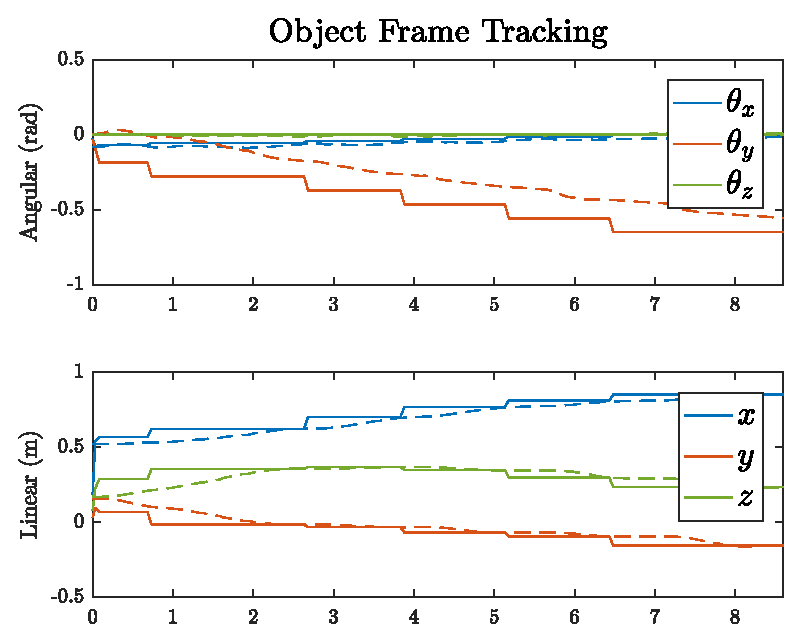
\includegraphics[width=0.46\textwidth]{images/singleAgent/exp11_objFrameTracking.eps}}%
	\hfill
	\subcaptionbox{\label{fig:exp11_ODN}}{%
		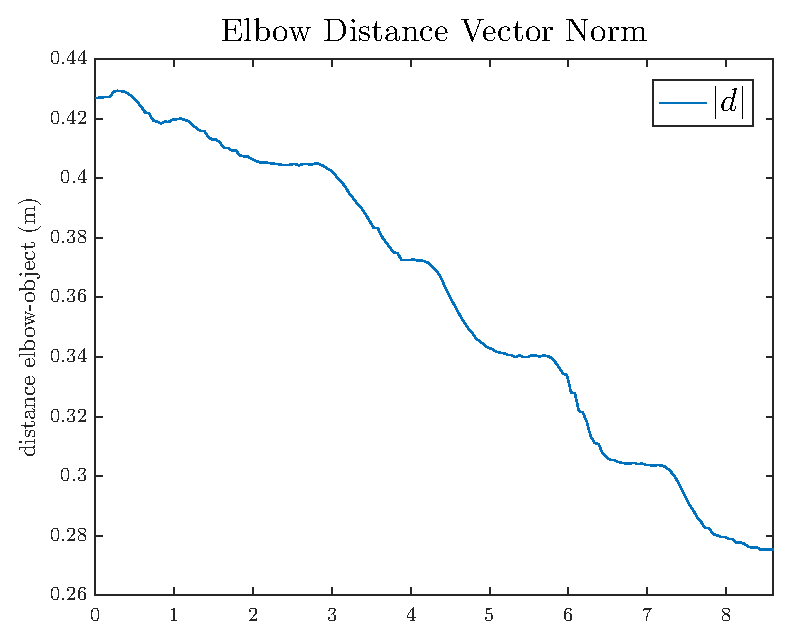
\includegraphics[width=0.46\textwidth]{images/singleAgent/exp11_objDistNorm.eps}}%
	\vspace{0.3cm}
	\subcaptionbox{\label{fig:exp10_OF}}{%
		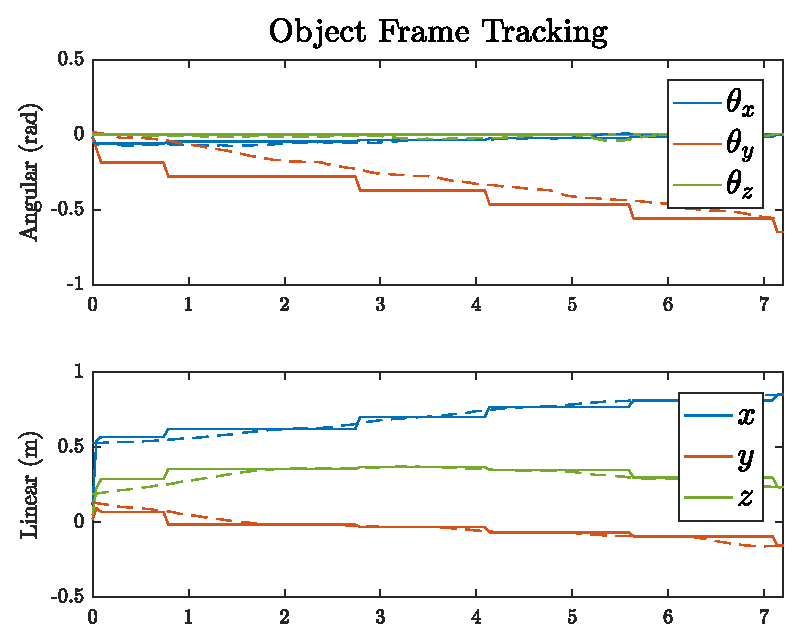
\includegraphics[width=0.46\textwidth]{images/singleAgent/exp10_objFrameTracking.eps}}%
	\hfill
	\subcaptionbox{\label{fig:exp10_ODN}}{%
		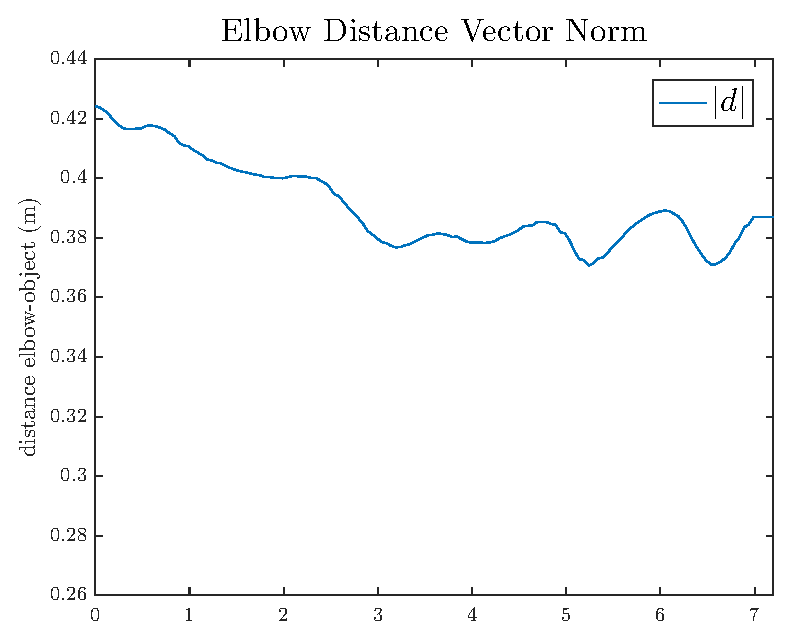
\includegraphics[width=0.46\textwidth]{images/singleAgent/exp10_objDistNorm.eps}}%
	\vspace{0.3cm}
	\subcaptionbox{\label{fig:exp10_EDA}}{%
		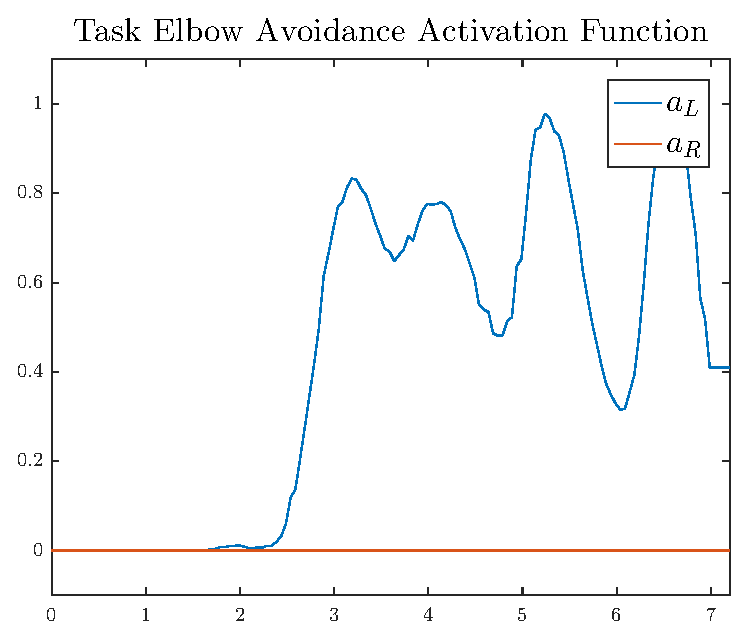
\includegraphics[width=0.435\textwidth]{images/singleAgent/exp10_elbDistA.eps}}%
	\hfill
	\subcaptionbox{\label{fig:ransac}}{%
		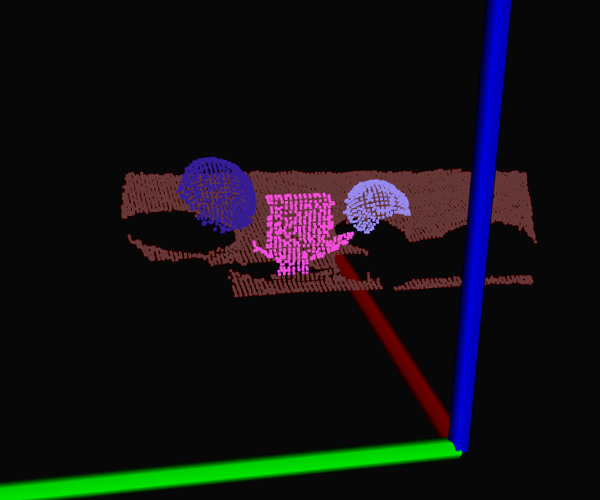
\includegraphics[trim={1cm 0 0 2.5cm},clip,width=0.45\textwidth]{images/singleAgent/ransac_frame.png}}%
	\caption{In figure \ref{fig:ransac} scene and objects recognized by OSP and relative frame of the vision system, each colour is identifying a different object. Figures \ref{fig:exp11_OF} and \ref{fig:exp11_ODN} are for the experiments with obstacle avoidance only at the HLL level and  figures  \ref{fig:exp10_OF}, \ref{fig:exp10_ODN} and \ref{fig:exp10_EDA} are for the experiments also with KCL reactive avoidance.}
	\label{fig:experiments}
	%\vspace{1.5cm}

%	\begin{subfigure}{}%{0.3\textwidth}
%		}	
%	\end{subfigure} 
%    \hfill
%	\begin{subfigure}{}%{0.3\textwidth}
%    \vspace{0.1cm}% Distancing the two rows of figures
%			
%	\end{subfigure}
%    \hfill
%	\begin{subfigure}{}%{0.3\textwidth}
%    \vspace{0.1cm}% Distancing the two rows of figures
%			
%	\end{subfigure}
%    \hfill
%    \begin{subfigure}{}%{0.285\textwidth}
%    \vspace{0.1cm}% Distancing the two rows of figures
%		
%	\end{subfigure}
%		\caption{In figure \ref{fig:ransac} scene and objects recognized by OSP and relative frame of the vision system, each color is identifying a different object. Figures \ref{fig:exp11_OF} and \ref{fig:exp11_ODN} are for the experiments with obstacle avoidance only at the HLL level and  figures  \ref{fig:exp10_OF}, \ref{fig:exp10_ODN} and \ref{fig:exp10_EDA} are for the experiments also with KCL reactive avoidance.}
%    \label{fig:experiments} 
%\end{figure*}